\documentclass[main.tex]{subfiles}

\begin{document}

\section{Bibliographien mit \LaTeX}


\begin{frame}[plain, fragile]
    \def\colorSetup{ForestGreen}
    \def\colorCompile{VioletRed}
    \def\colorBackend{DeepSkyBlue}

    \begin{center}
        \hspace*{-1cm}
        \begin{tikzpicture}
            [
            block/.style={rectangle, draw, minimum height=1cm, minimum width=2cm, align=center, thick},
            init/.style={initial by arrow, initial text=},
            arrow/.style={->,>=stealth},
            every initial by arrow/.style=arrow,
            every accepting by arrow/.style=arrow,
            ]

            % Frontend Nodes
            \node[block, init] (biblatex) {BibLaTeX};
            \node[block, init, below=6cm of biblatex] (natbib) {natbib};

            % Setup Nodes and their descriptions
            \node[block, below=2.25cm of biblatex.west, anchor=west, draw=\colorSetup] (setup biblatex) {Setup};
            \node[block, right=1.75cm of biblatex.north east, align=left, anchor=north west, draw=\colorSetup] (description setup biblatex) {\verb|\usepackage[backend=…]{biblatex}|\\\verb|\addbibresource{refs.bib}|};

            \node[block, above=2.25cm of natbib.west, anchor=west, draw=\colorSetup] (setup natbib) {Setup};
            \node[block, right=1.75cm of natbib.south east, align=left, anchor=south west, yshift=-0.4cm, draw=\colorSetup] (description setup natbib) {\verb|\usepackage{natbib}|\\\verb|\bibliographystyle{<style>}|\\\verb|\bibliography{refs.bib}|};

            % Compilation Nodes
            \node[block, right=0.7cm of setup biblatex, draw=\colorCompile] (1 compile biblatex) {1. Compile};
            \node[block, right=0.7cm of setup natbib, draw=\colorCompile] (1 compile natbib) {1. Compile};

            % Backend Nodes
            \node[block, right=1.25cm of 1 compile biblatex, draw=\colorBackend] (biber) {Biber};
            \node[block, right=1.25cm of 1 compile natbib, draw=\colorBackend] (bibtex) {BibTeX};

            % Last Compilation nodes
            \node[block, right=2.1cm of $(biber)!0.5!(bibtex)$, accepting by arrow, draw=\colorCompile] (2 compile) {2. Compile};


            % Arrows
            \draw[arrow] (biblatex) -- (setup biblatex);
            \draw[arrow] (natbib) -- (setup natbib);

            \draw[arrow] (setup biblatex) --  (1 compile biblatex);
            \draw[arrow] (setup natbib) -- (1 compile natbib);

            \draw[arrow] (1 compile biblatex) -- node[above] {.aux} node[below] {.bcf} (biber);
            \draw[arrow] (1 compile biblatex) -- node[above right=-0.1] {.aux} (bibtex);
            \draw[arrow] (1 compile natbib) -- node[above] {.aux} (bibtex);

            \draw[arrow] ($(biber.east)!0.5!(biber.south east)$) -- node[above right=0.1cm, xshift=-0.3cm] {.bbl} ($(2 compile.west)!0.5!(2 compile.north west)$);
            \draw[arrow] ($(bibtex.east)!0.5!(bibtex.north east)$) -- node[below right=0.1cm, xshift=-0.3cm] {.bbl} ($(2 compile.west)!0.5!(2 compile.south west)$);

        \end{tikzpicture}


    \end{center}
\end{frame}

\begin{frame}{Bibliographien mit \LaTeX{}: Backends im Vergleich}
    \begin{tabularx}{\textwidth}{L{100pt}*{2}{>{\centering\arraybackslash}X}}
        \toprule
        & Bib\TeX                                               & biber             \\\midrule
        Programmiersprache & C                                                   & Perl              \\
        Geschwindigkeit    & \href{https://tex.stackexchange.com/a/53302}{Schnell} & Langsam           \\
        Unicode support    & \cross                                                & \check            \\
        Datumsformat       & Eingeschränkt                                         & Flexibel          \\
        Sortierung         & Einfach                                               & Benutzerdefiniert \\
        Namensformatierung & Begrenzt                                              & Erweitert         \\
        \bottomrule
    \end{tabularx}
    \pause
    \begin{center}
        Was soll ich verwenden? → \href{https://tex.stackexchange.com/a/25702}{biber}
    \end{center}
\end{frame}

\begin{frame}[plain, fragile]
    \def\colorSetup{ForestGreen}
    \def\colorCompile{VioletRed}
    \def\colorBackend{DeepSkyBlue}

    \begin{center}
        \hspace*{-1cm}
        \begin{tikzpicture}
            [
            block/.style={rectangle, draw, minimum height=1cm, minimum width=2cm, align=center, thick},
            init/.style={initial by arrow, initial text=},
            arrow/.style={->,>=stealth},
            every initial by arrow/.style=arrow,
            every accepting by arrow/.style=arrow,
            ]

            % Frontend Nodes
            \node[block, init] (biblatex) {BibLaTeX};
            \node[block, init, below=6cm of biblatex] (natbib) {natbib};

            % Setup Nodes and their descriptions
            \node[block, below=2.25cm of biblatex.west, anchor=west, draw=\colorSetup] (setup biblatex) {Setup};
            \node[block, right=1.75cm of biblatex.north east, align=left, anchor=north west, draw=\colorSetup] (description setup biblatex) {\verb|\usepackage[backend=…]{biblatex}|\\\verb|\addbibresource{refs.bib}|};

            \node[block, above=2.25cm of natbib.west, anchor=west, draw=\colorSetup] (setup natbib) {Setup};
            \node[block, right=1.75cm of natbib.south east, align=left, anchor=south west, yshift=-0.4cm, draw=\colorSetup] (description setup natbib) {\verb|\usepackage{natbib}|\\\verb|\bibliographystyle{<style>}|\\\verb|\bibliography{refs.bib}|};

            % Compilation Nodes
            \node[block, right=0.7cm of setup biblatex, draw=\colorCompile] (1 compile biblatex) {1. Compile};
            \node[block, right=0.7cm of setup natbib, draw=\colorCompile] (1 compile natbib) {1. Compile};

            % Backend Nodes
            \node[block, right=1.25cm of 1 compile biblatex, draw=\colorBackend] (biber) {Biber};
            \node[block, right=1.25cm of 1 compile natbib, draw=\colorBackend] (bibtex) {BibTeX};

            % Last Compilation nodes
            \node[block, right=2.1cm of $(biber)!0.5!(bibtex)$, accepting by arrow, draw=\colorCompile] (2 compile) {2. Compile};


            % Arrows
            \draw[arrow, red, thick] (biblatex) -- (setup biblatex);
            \draw[arrow] (natbib) -- (setup natbib);

            \draw[arrow, red, thick] (setup biblatex) --  (1 compile biblatex);
            \draw[arrow] (setup natbib) -- (1 compile natbib);

            \draw[arrow, red, thick] (1 compile biblatex) -- node[above, black] {.aux} node[below, black] {.bcf} (biber);
            \draw[arrow] (1 compile biblatex) -- node[above right=-0.1] {.aux} (bibtex);
            \draw[arrow] (1 compile natbib) -- node[above] {.aux} (bibtex);

            \draw[arrow, red, thick] ($(biber.east)!0.5!(biber.south east)$) -- node[above right=0.1cm, xshift=-0.3cm, black] {.bbl} ($(2 compile.west)!0.5!(2 compile.north west)$);
            \draw[arrow] ($(bibtex.east)!0.5!(bibtex.north east)$) -- node[below right=0.1cm, xshift=-0.3cm] {.bbl} ($(2 compile.west)!0.5!(2 compile.south west)$);

        \end{tikzpicture}


    \end{center}
\end{frame}

\begin{frame}[fragile]{Bibliographien mit \LaTeX{}: Wie zitiere ich?}
    \begin{table}[H]
        \centering
        \begin{tabularx}{\textwidth}{{>{\ttfamily}L{130pt}X}}
            \toprule
            \textbf{Command}                 & \textbf{Output}           \\
            \midrule
            \textbackslash cite\{…\}         & \cite{TeXBook}            \\
            \textbackslash textcite\{…\}     & \textcite{BibLaTeXManual} \\
            \textbackslash parencite\{…\}    & \parencite{BeamerManual}  \\
            \textbackslash autocite\{…\}     & \autocite{TeXBook}        \\
            \textbackslash footcite\{…\}     & \footcite{TeXBook}        \\
            \textbackslash footfullcite\{…\} & \footfullcite{TikzManual} \\
            \bottomrule
        \end{tabularx}
        \caption{Zitationen im Stil der IEEE}
        \label{tab:DifferentWaysOfCiting}
    \end{table}
\end{frame}

% Due to the nature of biblatex / biber, it is not possible to use multiple citation styles in one document. Thus, these PDF slides have been generated and extracted seperately.
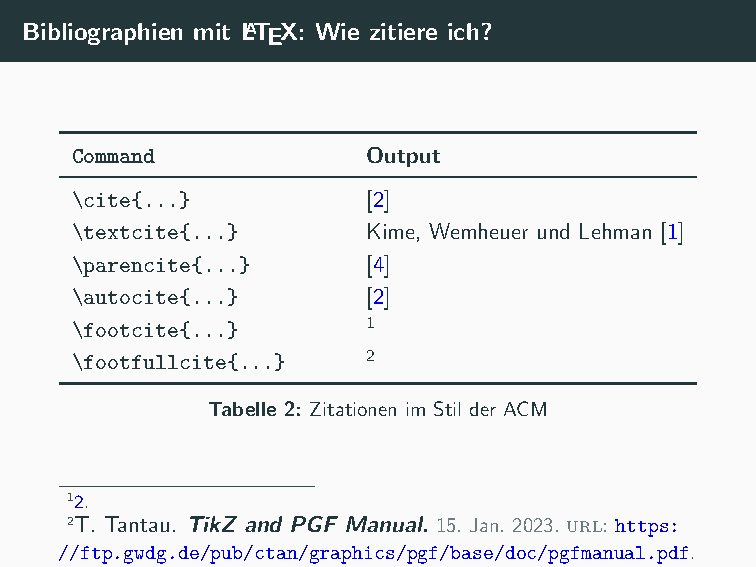
\includepdf{CitationStyles/acm-style.pdf}
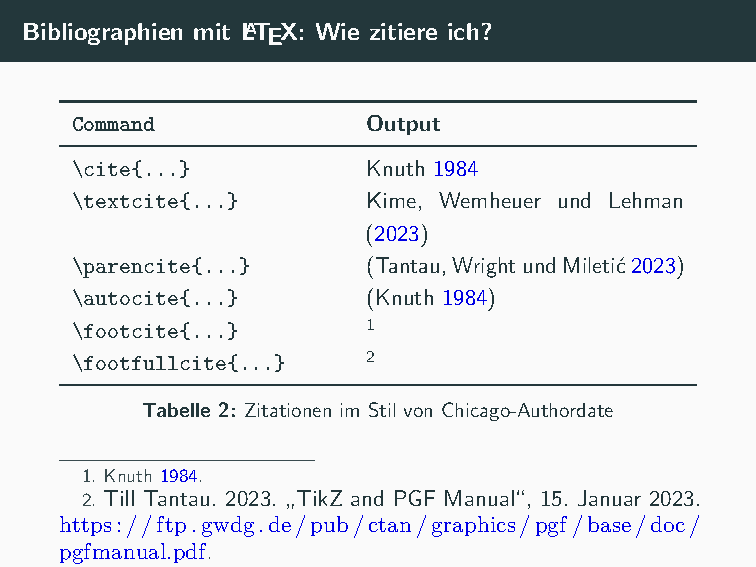
\includepdf{CitationStyles/chicago-style.pdf}
\includepdf{CitationStyles/apa-style.pdf}


\begin{frame}{Bibliographien mit \LaTeX{}: Quellenverzeichnis}
    \printbibliography[heading=none]
\end{frame}


\end{document}